%%%%%%%%%%%%%%%%%%%%%%%%%%%%%%%%%%%%%%%%%%%%%%%%%%%%%%%%%%%%%%%%%%%%%%%%%%%%%%%%
%2345678901234567890123456789012345678901234567890123456789012345678901234567890
%        1         2         3         4         5         6         7         8

\documentclass[letterpaper, 10 pt, conference]{ieeeconf}  % Comment this line out if you need a4paper

%\documentclass[a4paper, 10pt, conference]{ieeeconf}      % Use this line for a4 paper

\IEEEoverridecommandlockouts                              % This command is only needed if 
                                                          % you want to use the \thanks command

\overrideIEEEmargins                                      % Needed to meet printer requirements.

% See the \addtolength command later in the file to balance the column lengths
% on the last page of the document

% The following packages can be found on http:\\www.ctan.org
\usepackage{float}
\usepackage{graphicx} % for pdf, bitmapped graphics files
%\usepackage{epsfig} % for postscript graphics files
%\usepackage{mathptmx} % assumes new font selection scheme installed
%\usepackage{times} % assumes new font selection scheme installed
%\usepackage{amsmath} % assumes amsmath package installed
%\usepackage{amssymb}  % assumes amsmath package installed

\title{\LARGE \bf
Exoskeletons
}


\author{Aydin Tekin$^{1}$% <-this % stops a space
\thanks{*This work was not supported by any organization}% <-this % stops a space
\thanks{$^{1}$Aydin Tekin is student at the Karlsruhe Institute of Technology, 76131 Karlsruhe, Germany
        {\tt\small aydin.tekin@student.kit.edu}}%
}


\begin{document}



\maketitle
\thispagestyle{empty}
\pagestyle{empty}


%%%%%%%%%%%%%%%%%%%%%%%%%%%%%%%%%%%%%%%%%%%%%%%%%%%%%%%%%%%%%%%%%%%%%%%%%%%%%%%%
\begin{abstract}

In the last decades, the research in the field of exoskeletons led to systems which due the durability and
user-friendliness are capable of assisting humans in many aspects. The idea of augmenting human strength and
alleviating human deficiencies led to great efforts in the realization of such systems. In this paper, the current
"state of art" and the key functionalities of exoskeletons will be presented.

\end{abstract}


%%%%%%%%%%%%%%%%%%%%%%%%%%%%%%%%%%%%%%%%%%%%%%%%%%%%%%%%%%%%%%%%%%%%%%%%%%%%%%%%

\section{INTRODUCTION}

One way how an exoskeletons is defined, can be described with the following sentence:
"A [...] structure, [...], that provides protection or support for an organism."
The use-cases of an exoskeleton can be divided into three main sectors: military, medicine, and industry.

%%%%%%%%%%%%%%%%%%%%%%%%%%%%%%%%%%%%%%%%%%%%%%%%%%%%%%%%%%%%%%%%%%%%%%%%%%%%%%%%

The biggest of these three sectors is the military sector.
Pursuing the vision of increasing the strength and durability of american soldiers, the US Department of Defence
started with the development of exeoskeletons in the early 60's. The first prototype, the "Hardiman", which has been presented by
General Electric featured a weight of more than 750 kg and the capability of lifting loads up to 250 kg.
Due the fact that at that time only a single arm could be controlled and that the arm was only capable of lifting
a third of its own weight, the prototype proved to be ineffecient. Thus, the research on this prototype has been
discontinued. As a result, the DARPA (Defense Advanced Research Projects Agency) fortified their cooperations with
research facilities in order to enforce the research on exoskeletons for military purposes. The progress in this area
led to prototypes like BLEEX (Berkeley Lower Extremity EXoskeleton). Seeing the future potential of these prototypical
designs, private companies bought most of the licenses of these prototypes in order to continue the development
of these systems. An exemplary result is the HULC (Human Universal Load Carrier) which is actively developed and produced
by Lockheed Martin, and, thus, is an excellent example for these kind of commercialised systems.

%%%%%%%%%%%%%%%%%%%%%%%%%%%%%%%%%%%%%%%%%%%%%%%%%%%%%%%%%%%%%%%%%%%%%%%%%%%%%%%%

The medical sector is the second biggest one; the first prosthesis has been crafted in ancient Egypt (600 B.C.)
in the form of a wooden toe. Centuries later, these kind of prostheses were continually enhanced but still remained
artificial parts of static nature. After two world wars, the demand of prostheses for limbs increased dramatically,
researchers were urged to work on systems capable of emulating the functionality of the human limbs. Another factor
is the demographic change in industrialized countries, affected by good medical care and lower mortality rate leading
to a growing percentage of elderly and disabled people. This forced the medicine to create systems to support and
ensure a certain quality of life for these people.

%%%%%%%%%%%%%%%%%%%%%%%%%%%%%%%%%%%%%%%%%%%%%%%%%%%%%%%%%%%%%%%%%%%%%%%%%%%%%%%%

Also the industry is seeking for years for systems to support workers to finish their work faster and more efficiently.
In the agricultural sector or manufacturing, where workers have to perform simple movements in repetitive manner,
exoskeletons could grant the users more durability und less workload. Also safety is a very important aspect in this field.
Workers who carry heavy or dangerous materials should have a reliable system assisting them in their daily
work.

Great interest in the possibilities provided by exoskeletons has been shown in the entertainment sector as well.
This fact will be discussed later.

%%%%%%%%%%%%%%%%%%%%%%%%%%%%%%%%%%%%%%%%%%%%%%%%%%%%%%%%%%%%%%%%%%%%%%%%%%%%%%%%

The question how to design a modern exoskeleton has been addressed by the various research groups and companies. The
design principles vary according to the intended use-case. However, common to all modern designs is the requirement for a
user-friendly, intuitive, and safe handling. A important key to achieve this, is by increasing the acceptance of the
system from the perspective of the human user by raising the level of comfortability, agility, and usability provided
by the system. 



\section{STATE OF THE ART}

The different systems presented in this paper can be divided into three general categories: lower body, upper body, and
full body exoskeletons.

%%%%%%%%%%%%%%%%%%%%%%%%%%%%%%%%%%%%%%%%%%%%%%%%%%%%%%%%%%%%%%%%%%%%%%%%%%%%%%%%

Lower body exoskeletons are mostly designed for the medical sector. The most common use is for rehabilitation of people
with deficiencies such as a pathological walking pattern (e.g. caused by long-term confinement in bed or by vestibular
disorder). Some of these systems even go a step further and try to give disabled people some amount of their mobility
back.

%%%%%%%%%%%%%%%%%%%%%%%%%%%%%%%%%%%%%%%%%%%%%%%%%%%%%%%%%%%%%%%%%%%%%%%%%%%%%%%%

Upper body exoskeletons have different application areas. The XOS 2 for example is planned to be used on military
operations whereas other systems aim to be used in the industry. Applied the entertainment industry, on can think of
an exoskeleton as an addition to a VR-headset to create an even more authentic virtual reality experience. In
manufacturing, exoskeletons can be used to teleoperate robotic systems in order to deal with hazardous materials e.g.
in the chemical industry.

%%%%%%%%%%%%%%%%%%%%%%%%%%%%%%%%%%%%%%%%%%%%%%%%%%%%%%%%%%%%%%%%%%%%%%%%%%%%%%%%

The last category are the full body exoskeletons which are designed for the assistance of the whole body.
Common applications are augmentation of human power which allows the lifting and the transport ofheavy objects.
For example, the HULC (Human Universal Load Carrier) helps soldiers to carry more supplies on the battlefield.
Other systems assist people in their daily life or work.

%%%%%%%%%%%%%%%%%%%%%%%%%%%%%%%%%%%%%%%%%%%%%%%%%%%%%%%%%%%%%%%%%%%%%%%%%%%%%%%%

Altough the following systems were initially designed for a special purpose, due to continuous developement,
there are systems which cannot be clearly associated to one of the mentioned categories. For example, the HAL
(Hybring Assistive Limb) was firstly developed as lower body exoskeleton. However, the second generation has been extended
by an upper body component yielding a full body solution. Hence, the categorization of exoskeletons is
not strict, and, thus, certain systems can be assigned to multiple categroies.

\subsection{Lower body exoskeletons}

E-Legs have been originally created by Berkeley Bionics in the USA which was later renamed to Ekso Bionics. In this context,
the exoskeleton has been renamed to Ekso as well. Powered by a battery, attached at the back of the exoskeleton, it can run
up to 6 hours. It is used for rehabilitation purposes, mostly for people with walking disabilities. With a self-learing
algorithm an adapted system control is implemented which requires the daily training over several weeks daily of the user
until they can independantly stand up from their wheel-chair and walk freely. Even if the system is still slow and the
walking movements are not very smooth, it gives wheel-chair confined people a great amount of mobility and freedom.
This system was commercialized several years ago and is currently used in rehabilitation centers and costs around 100,000 US-Dollar. \newline

%%%%%%%%%%%%%%%%%%%%%%%%%%%%%%%%%%%%%%%%%%%%%%%%%%%%%%%%%%%%%%%%%%%%%%%%%%%%%%%%

\begin{figure}[H]
  \centering
    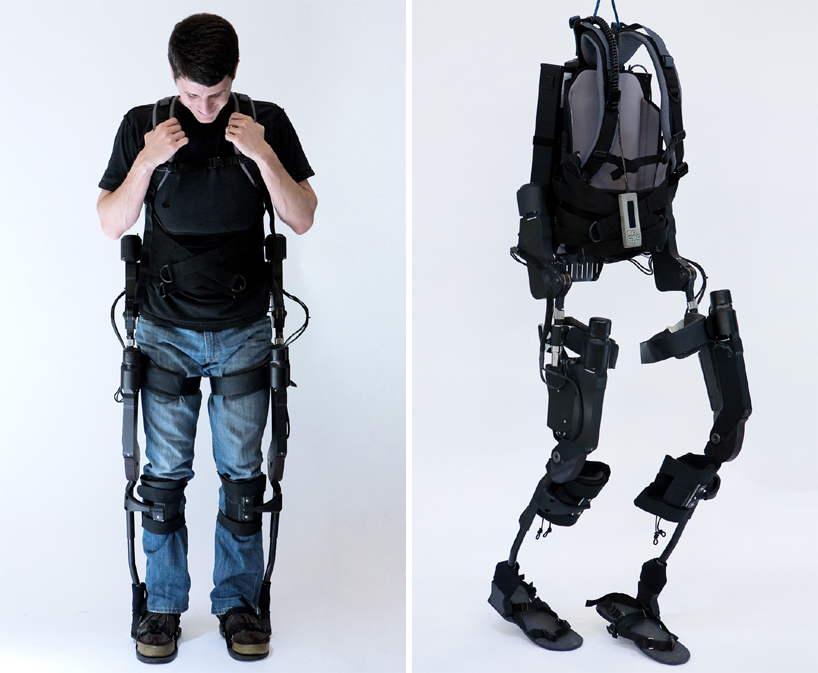
\includegraphics[width=0.5\textwidth]{img/elegs}
  \caption{E-Legs/Ekso by Ekso Bionics, USA}
\end{figure}

%%%%%%%%%%%%%%%%%%%%%%%%%%%%%%%%%%%%%%%%%%%%%%%%%%%%%%%%%%%%%%%%%%%%%%%%%%%%%%%%

LOPES (LOwer Powered ExoSkeleton) is being developed by the University of Twente in the Netherlands and is a stationary
exoskeleton. Similar to the Ekso system, it is used for rehabilitation where the main difference is that this system
is tethered and mostly controlled by a second operator sitting behind the computer attached to the exoskeleton.
The target groups are not disabled people but patients who suffered from muscle atrophy which might have been caused
by longer bedriddenness or by vestibular disorder. The patients are individually trained by the system
hich collectes data on the fly. Depending on the data, the operator can then tune the system to give the user
more freedom or assist him more with walking. Each leg incorporates 8 DoF. Thus, LOPES grants full flexibility and
a very natural walking flow for the user.\newpage

%%%%%%%%%%%%%%%%%%%%%%%%%%%%%%%%%%%%%%%%%%%%%%%%%%%%%%%%%%%%%%%%%%%%%%%%%%%%%%%%

\begin{figure}[H]
  \centering
    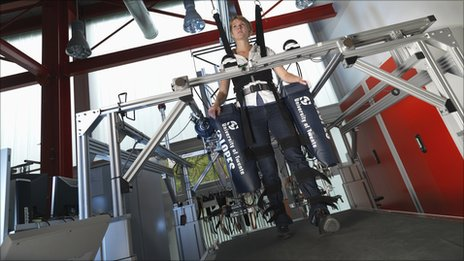
\includegraphics[scale=1.1]{img/lopes}
  \caption{LOPES by University of Twente, Netherlands}
\end{figure}

%%%%%%%%%%%%%%%%%%%%%%%%%%%%%%%%%%%%%%%%%%%%%%%%%%%%%%%%%%%%%%%%%%%%%%%%%%%%%%%%

The Honda Walking Assist is a lightweight lower extremity exoskeleton developed and maintained by Honda Motor Co., Ltd. in Japan.
With a total weight of 2.6 kg (including battery) it is a very mobile device running up to 4 hours with one charge.
The battery is also very small and is attached at the back of the device similar to the ELegs. Originally it has been
designed to be used by workers in Honda production centers to assist them in their work. Extending the application areas,
it is further used in daily life for disabled and elderly people having mobility difficulties, for example walking upstairs.
After 16 years of developement and evaluation, it is used in about 50 hospitals all around Japan and can be leased
by companies.

%%%%%%%%%%%%%%%%%%%%%%%%%%%%%%%%%%%%%%%%%%%%%%%%%%%%%%%%%%%%%%%%%%%%%%%%%%%%%%%%

\begin{figure}[H]
  \centering
    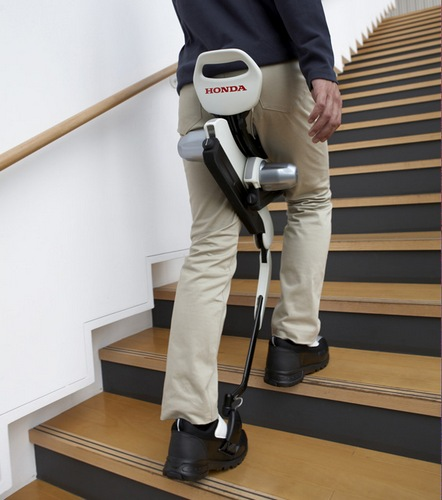
\includegraphics[scale=0.5]{img/honda}
  \caption{Honda Walking Assists by Honda Motor, Japan}
\end{figure}
\newpage

%%%%%%%%%%%%%%%%%%%%%%%%%%%%%%%%%%%%%%%%%%%%%%%%%%%%%%%%%%%%%%%%%%%%%%%%%%%%%%%%

\subsection{Upper body exoskeletons}

ExoHand is a commercial product distributed by Festo Corporate in Germany. Like LOPES it is a tethered system and
uses only a component for the hand. One of its key-features is the force-feedback system, which opens the system to
new use-cases. Initially, it has been designed designed for industrial use. It is used as a remote interface to
work with risky materials offering the operators maximum freedom grades by controling a five-fingered remote hand.
Furthermore, the force-feedback system allows the creation virtual environments in which one can operate with the hand.
In addition to a virtual reality headset, realistic games can be created where the user does not just see a virtual
world but also can feel and operate in it. In its very extendible and modular nature, researchers created a brain
computer interface which paved the way to medical use-cases. Patients who had an apoplexy can be trained with it.
In this way, the link between hand to brain activities which might be interrupted and damaged can be partially recovered.

%%%%%%%%%%%%%%%%%%%%%%%%%%%%%%%%%%%%%%%%%%%%%%%%%%%%%%%%%%%%%%%%%%%%%%%%%%%%%%%%

\begin{figure}[H]
  \centering
    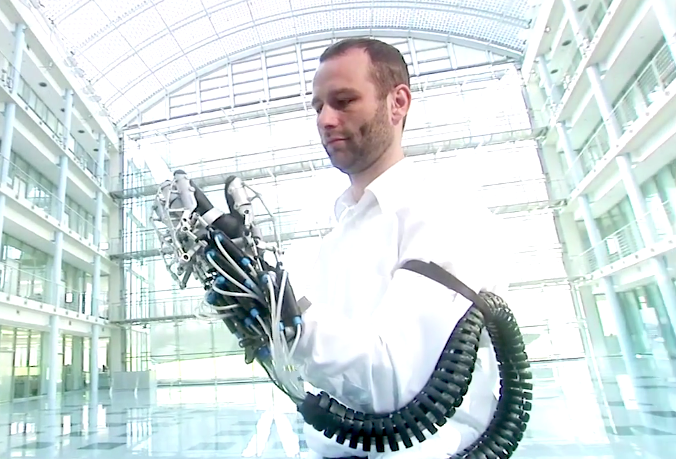
\includegraphics[width=0.5\textwidth]{img/exohand}
  \caption{ExoHand by Festo, Germany}
\end{figure}

%%%%%%%%%%%%%%%%%%%%%%%%%%%%%%%%%%%%%%%%%%%%%%%%%%%%%%%%%%%%%%%%%%%%%%%%%%%%%%%%

XOS 2 initially developed by Sarcos was later on bought up by Raytheon, USA. In the year 2000, DARPA requested for
military exoskeleton and XOS could enfore against 14 other exemplars. It is fully designed for military use and
contains two components: the main upper extremity component and the lower extremity component. The exoskeleton
enables the user to lift up to 90 kg and to break through wooden boards. According to the specifications, it is assumed
that the soldiers wearing the XOS can have the performance three soldiers in the battle field. On the one hand, the XOS
features a high agilitiy, on the other hand, the main disadvantage of is that it still tethered to a station
since no mobile power source could be found which can provide enough power for the suit. The US Army is still
doing tests and it is expected that it enters military service by the year 2015, although, it is not expected
to have a working untethered version until 2020.

\newpage

\begin{figure}[H]
  \centering
    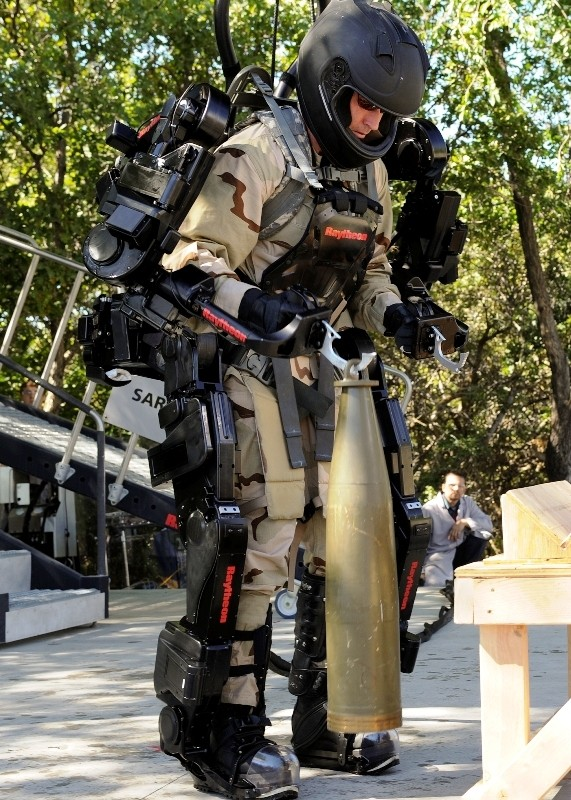
\includegraphics[width=0.4\textwidth]{img/xos2}
  \caption{XOS 2 by Sarcos/Raytheon, USA}
\end{figure}

\subsection{Full body exoskeletons}

BLEEX (Berkeley Lower Extremity Exoskeleton) is a full body exoskeleton funded by the DARPA for military purposes
in 2001 and developed by the University of California, USA. Powered by a battery, it was back then the fastest
exoskeleton featured speeds up to 2m/s but this design also had its downsides. It could only run up to 3 hours which
made it very unpractical to use it in the battlefield. But granting the user 7 DoF only on the legs,
a very agile system has been developed which allows soldiers to wear this exoskelton while walking through bumpy fields
without any limitations. Furthermore, it could lift up to 75 kg without the user noticing it allowing soldiers
to carry much more weight, lift up heavy projectiles and be much more durable.
With a total weight of 17 kg it can be easily transported and is very mobile. Because of its high potential it was
later bought by Lockheed Martin. \newpage

%AB HIER BITTE NACHBEARBEITEN !!!
%%%%%%%%%%%%%%%%%%%%%%%%%%%%%%%%%%%%%%%%%%%%%%%%%%%%%%%%%%%%%%%%%%%%%%%%%%%%%%%%

\begin{figure}[H]
  \centering
    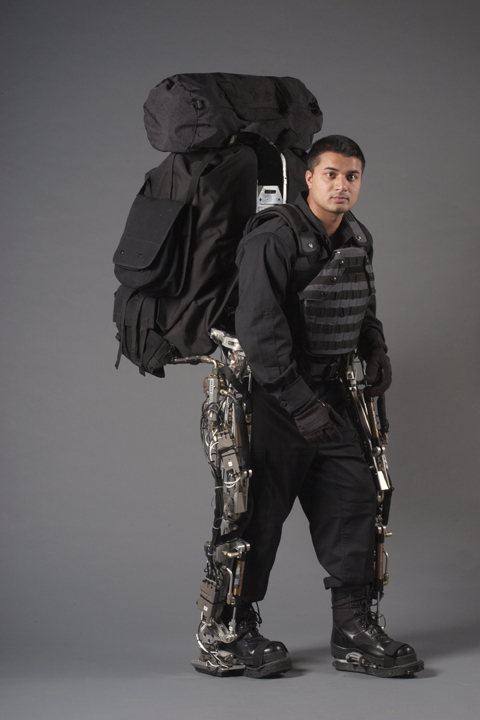
\includegraphics[width=0.4\textwidth]{img/bleex}
  \caption{BLEEX by University of California, USA}
\end{figure} 

%%%%%%%%%%%%%%%%%%%%%%%%%%%%%%%%%%%%%%%%%%%%%%%%%%%%%%%%%%%%%%%%%%%%%%%%%%%%%%%%

HULC (Human Universal Load Carrier) is the descendant of BLEEX and is actively developed by Lockheed Martin,
USA since 2009. It is a mobile, untethered system and like his ancestor it is currently powered by a battery but
has a longer duration; the whole system was redesigned and ligther, more efficient components were used for the
exoskeleton. Now one charge can power the suit up to 8 hours. In comparison to Figure 6 in Figure 7 you can see
that the researchers of Lockheed Martin set great value in simplifying and optimizing the architecture and the material used for the exoskeleton. But this doesn't mean that the system got 'weaker' now; even if the material got ligther a new hydraulic system was implemented allowing the HULC to lift up to 90 kg (15 kg more than BLEEX). The sensors are now placed on the foot pads relaying the information to the onboard controller who then estimates the movements. This way the soliders have the ability to run, crawl or even squat. Additionally mobility was improved; it can now be put on in a few minutes and can be later easily folded to a very compact package. With a great funding by the US Department of Defence and US Army Natick Soldier Research Development and Engineering Center it was tested on real environments and recently been evaluted by these two institutions, so its expected to be used in the real battlefield by 2016. Recently Lockheed Martin announced its evaluating a new fuel cell power source massively increasing the operation time up to 98 hours.\newpage

%%%%%%%%%%%%%%%%%%%%%%%%%%%%%%%%%%%%%%%%%%%%%%%%%%%%%%%%%%%%%%%%%%%%%%%%%%%%%%%%

\begin{figure}[H]
  \centering
    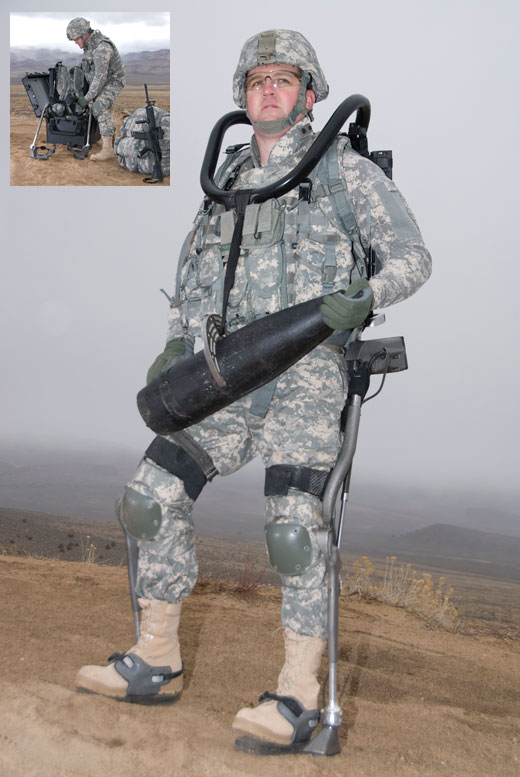
\includegraphics[width=0.4\textwidth]{img/hulc}
  \caption{HULC by Lockheed Martin, USA}
\end{figure}

%%%%%%%%%%%%%%%%%%%%%%%%%%%%%%%%%%%%%%%%%%%%%%%%%%%%%%%%%%%%%%%%%%%%%%%%%%%%%%%%

The HAL-5 (Hybrid Assistive Limb) is a research project in cooperation between the Tskuba university and Cyberdye Inc., Japan. The project was initated by Yoshiyuki Sankai in 1994; in the first versions it was wired to a external computer and was very inefficent and slow. With the progress on faster and smaller processors and also with the more and more optimised power sources, the third generation of HAL was the first mature prototype and was presented in the early 2000s. It only had a lower body component and was still very unpractical. So the researchers intensified to work on a upper body component and the result was the HAL 5, which weighted much less than the previous versions but was much more powerfull. By now it weighted only 10 kg and could lift up to 70 kg. Additionally the knees were supported by the suit and so the users could leg-press up to 180 kg. With a duration time 4 to 5 hours its still very inefficent but Cyberdyne intensively works on extending it. The suit uses EMG-signals to gather information about the users movement placed all over the body. It has two different modes to support the user; the first one is user-activated, the second one is robotic controlled to achieve continuous automatic user motions. But this system complicates putting on the device, so a technical experienced helper is needed to place the sensors in the right place.

%%%%%%%%%%%%%%%%%%%%%%%%%%%%%%%%%%%%%%%%%%%%%%%%%%%%%%%%%%%%%%%%%%%%%%%%%%%%%%%%

It's also the first exoskeleton which was certified with ISO 13485 – an international quality standard for medical devices. So it was distributed to hundreds of hostpitals and rehabilitation centers all over Japan to help nurses in their work. The system received international attention when the suit was used to salvage operation at the destroyed fukushima atom reactor. For this purpose Cyberdyne customized and enhanced the suit to be durable to radiation. In addition to that its also planned to be used in the industry to support workers in the agricultural sector. 

%%%%%%%%%%%%%%%%%%%%%%%%%%%%%%%%%%%%%%%%%%%%%%%%%%%%%%%%%%%%%%%%%%%%%%%%%%%%%%%%

\begin{figure}[H]
  \centering
    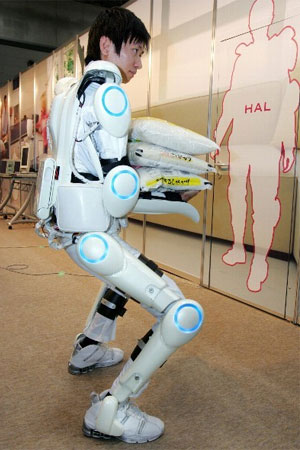
\includegraphics[width=0.4\textwidth]{img/hal}
  \caption{HAL-5 by Cyberdyne, Japan}
\end{figure}

%%%%%%%%%%%%%%%%%%%%%%%%%%%%%%%%%%%%%%%%%%%%%%%%%%%%%%%%%%%%%%%%%%%%%%%%%%%%%%%%

\section{DISSCUSION}

Altough the presented systems are very advanced, there are still difficulties the researchers have to face developing efficient systems. 

%%%%%%%%%%%%%%%%%%%%%%%%%%%%%%%%%%%%%%%%%%%%%%%%%%%%%%%%%%%%%%%%%%%%%%%%%%%%%%%%

The sensor technology is still not as advanced as we think. Many systems still dont use any active sensors to to obtain human body signals, instead passive sensors measure the movement initiated by the human then try to estimate the future movement and then react to this. This has the advantage that you can easily put on the exoskeleton without having to place sensors accuratetly on defined spots on your body. But the kind of sensor system is very inaccurate and reacts pretty slowly to human interaction, which may restrict the agility of the user. Some systems use Electromyography, detecting eletrical potential generated by muscels, using EMG-Sensors on the skin of the user to analyse the movement of him. Even if we get much better results, they are still very inaccurate because we cant "dock" directly on the muscle cells. Additionally it is very difficult for a normal user to put on these kind of exoskeletons because you need an experienced assistant to put the sensors to the right spot on the body. Any deviantions could have an immense influence of the algorithm used for motion detection. Currently researchers are trying to optimize the existing sensors but also are working on other ways to obtain human signals like using EMG-needles.

%%%%%%%%%%%%%%%%%%%%%%%%%%%%%%%%%%%%%%%%%%%%%%%%%%%%%%%%%%%%%%%%%%%%%%%%%%%%%%%%

Security is also seen as an important feature in developing such systems. People who use this system must be able to trust them and the system should be "secure" otherwise the user could get injured in many ways. In the worst case the exoskeleton may wrench extremities of humans or could suddenly shutdown leaving the user back with a heavy load. That's why the researcher try to define guidelines for secure systems; one of them is ISO 13485. It covers different aspects of secure medical systems like corrective and preventive actions or risk management. HAL-5 is the first exoskeleton who has this certification and other systems are expected to follow.

%%%%%%%%%%%%%%%%%%%%%%%%%%%%%%%%%%%%%%%%%%%%%%%%%%%%%%%%%%%%%%%%%%%%%%%%%%%%%%%%

Most focus on the recent work is the question which power supply should be used and how it can be optimized. Some systems like XOS dont even use any autonomous power supplies, they are attached with wires to a station. This gives a full electrical durability but they can only be used stationary. For independant exoskeletons there are currently two different types of power supplies; the first one is using a battery which is attached to the exoskeleton. This solution has a very low capacity, so the systems can only work for a few hours which might be a very short length of time, depending on the use-case. Also batteries are heavy, recharging takes too much time and the durability of a battery decreases over time. Fuels are an alternative which can trump with a high and long-lasting energy output resulting in operating time of several days. Refilling can be done very fast and you dont have to find fixed stations to refill the energy source. But it also has its downsides, it's very noisy to use and very insecure: the content is highly flammable. The HAL-5 uses a highly optimized battery and can work up to 5 hours with one charge, using it in an medical environment there is no way to use noisy and smoking energy sources. HULC is planned to use a fuel based power supply, its important for these kind of military-used exoskeletons to have a large operation time. Until there is no other good alternative, one of the mentioned types have to be used and the disadvantes have to be accepted.
 

\section{CONCLUSION}

The human body has flaws and limitations which will and have to be fixed with the increasing technical possibilites we have. With exoskeletons, it seems like a solution for this problem is found, so the work on improving must be intensified.

%%%%%%%%%%%%%%%%%%%%%%%%%%%%%%%%%%%%%%%%%%%%%%%%%%%%%%%%%%%%%%%%%%%%%%%%%%%%%%%%

Companies understood the importance of this sector and started commercializing products, which to then just were seen as objects in research. Evermore exoskeletons are made accessible to the general public this way, even if the prices are still too high for the most people to buy them.

%%%%%%%%%%%%%%%%%%%%%%%%%%%%%%%%%%%%%%%%%%%%%%%%%%%%%%%%%%%%%%%%%%%%%%%%%%%%%%%%


\begin{thebibliography}{99}

\bibitem{c1} Brown, P., Jones, D., Singh, S. K., and Rosen, J. M., The exoskeleton glove for control of paralyzed hands.In Proceedings of the IEEE 
International Conference on Robotics and Automation, Atlanta, GA, USA, 1993, vol. 1,pp. 642-647.
\bibitem{c2} Robert Bogue, Exoskeletons and robotic prosthetics: a review of recent developments, 2009
\bibitem{c3} Dollar A.M., Herr H., Lower extremity exoskeletons and active orthoses: challenges and state-of-the-art, 2008
\bibitem{c4} Guizzo E., Goldstein H., The rise of the body bots [robotic exoskeletons], 2005
\bibitem{c5} Shigeo Tanabe, Satoshi Hirano, Eiichi Saitoh, Wearable Power-Assist Locomotor (WPAL) for supporting upright walking in persons with paraplegia, 2013
\bibitem{c6} Zoss A., Kazerooni H., Chu A., On the mechanical design of the Berkeley Lower Extremity Exoskeleton (BLEEX), 2005 
\bibitem{c7} Kazerooni H., Exoskeletons for human power augmentation, 2005
\bibitem{c8} Naruse, K., Kawai, S., Yokoi, H., and Kakazu, Y. Devel-opment of wearable exoskeleton power assist sys-tem for lower back support. In Proceedings of theIEEE/RSJ International Conference on Intelligent Robotsand Systems, Las Vegas, Nevada, USA, 2003, vol. 3,pp. 3630-3635.
\bibitem{c9} Pratt J.E., Krupp B.T., Morse C.J., Collins S.H., The RoboKnee: an exoskeleton for enhancing strength and endurance during walking, 2004
\bibitem{c10} Veneman J.F., Kruidhof R., Hekman E.E.G., Ekkelenkamp R., Design and Evaluation of the LOPES Exoskeleton Robot for Interactive Gait Rehabilitation, 2007
\bibitem{c11} Tsagarakis N. G., Caldwell Darwin G., Development and Control of a ?Soft-Actuated? Exoskeleton for Use in Physiotherapy and Training, 2003
\bibitem{c12} Banala S.K., Seok Hun Kim, Agrawal S.K., Scholz J.P., Robot Assisted Gait Training With Active Leg Exoskeleton (ALEX), 2008
\bibitem{c13} Gupta A., O'Malley M.K., Design of a haptic arm exoskeleton for training and rehabilitation, 2006 
\bibitem{c14} Walsh C.J., Paluska D., Pasch K., Grand W., Development of a lightweight, underactuated exoskeleton for load-carrying augmentation, 2006
\bibitem{c15} Koyama T., Yamano I., Takemura K., Maeno T., Multi-fingered exoskeleton haptic device using passive force feedback for dexterous teleoperation, 2002

\end{thebibliography}

\end{document}
